\documentclass[a4paper,12pt,DIV=12,BCOR=10mm,ngerman,twoside,openright]{scrreprt}	% Druck-Version mit kleinerem Rand für Bindung
% \documentclass[a4paper,12pt,DIV=12,ngerman]{scrreprt}

\raggedbottom % Fügt dies hinzu, um ungleichmäßige Seitenlängen zu erlauben
\usepackage{lmodern}

\usepackage[T1]{fontenc}						% europäische Kodierung: Umlaute im Fließtext
\usepackage[utf8]{inputenc}		 				% Eingabezeichensatz: Umlaute im Code
\usepackage[ngerman]{babel}						% Deutsches Sprachpaket mit Trennmuster
\usepackage[babel,german=quotes]{csquotes}		% Deutsche Anführungszeichen
\usepackage{scrlayer-scrpage}					% Eigene Kopf- und Fußzeilen
\usepackage{microtype}							% Optischer Randausgleich (vorher cm-super installieren)


% Globale Definitionen ------------------------------------------------------------------ %
\newcommand{\Titel}{Geiler Robi macht noch geilere Stunts}
\newcommand{\Fak}{Automatisierungstechnik}
\newcommand{\Datum}{\today}
\newcommand{\Name}{Stefan Sauerer, Bent Benjo, Lucy Lukas}
% --------------------------------------------------------------------------------------- %

% Grafiken und Plots -------------------------------------------------------------------- %
\usepackage{graphicx}							% Abbildungen einbinden
\usepackage{tikz}								% Vektorgrafiken
\usepackage{pgfplots}							% Daten plotten
\pgfplotsset{compat=1.18}
\usepackage{float}								% Bessere Plazierung der Bilder (H)

% --------------------------------------------------------------------------------------- %

% Tabellen ------------------------------------------------------------------------------ %
\usepackage{tabularx}							% Tabellen mit fester Breite
\usepackage{booktabs}							% Abstände in Tabellen
\usepackage{paralist}							% Flexible Aufzählungen
\usepackage{ltxtable}							% Lange Tabellen fester Breite
% --------------------------------------------------------------------------------------- %

% Zitieren ------------------------------------------------------------------------------ %
												% Optionen -> Erzeugen -> Biber auswählen
\usepackage[backend=biber]{biblatex}			% Literaturverzeichnis richtig darstellen
\addbibresource{Literatur.bib}					% BibTex Datei einbinden
% --------------------------------------------------------------------------------------- %
\usepackage{amsmath}

\usepackage{hyperref}							% Links in Gliederung einfügen

\usepackage{siunitx}							% Für SI einheiten
\sisetup{locale = DE}

% Farben definieren (Krones CI Farben ) ------------------------------------------------- %
\usepackage{xcolor}								% Farben selbst definieren
\definecolor{BasicBlue}              {HTML}{0060AD}
\definecolor{SolidBlue}              {HTML}{052A68}
\definecolor{SolidGreyLight}         {HTML}{EAEBEB}
\definecolor{SolidGreyDark}          {HTML}{B4BABE}
\definecolor{Silver}                 {HTML}{CCCCCC}
\definecolor{TextGrey}               {HTML}{555555}
\definecolor{AccentuationBlue}       {HTML}{66B0E2}
\definecolor{AccentuationBlueMuted}  {HTML}{6083A4}
\definecolor{AccentuationYellow}     {HTML}{FFDD00}
\definecolor{AccentuationYellowMuted}{HTML}{E0B000}
\definecolor{AccentuationOrange}     {HTML}{E34805}
\definecolor{SolidRed}               {HTML}{B3282E}
\definecolor{AccentuationRedMuted}   {HTML}{80333A}
\definecolor{AccentuationGreen}      {HTML}{97C218}
\definecolor{AccentuationGreenMuted} {HTML}{00987A} % Farben einbinden
% --------------------------------------------------------------------------------------- %

% Dokumentbeginn
\begin{document}
% Kopf- und Fußzeilen =================================================================== %
\pagestyle{scrplain}
\clearpairofpagestyles
\ofoot[\pagemark]{\pagemark}
\ihead{\headmark}
\automark{chapter}
\pagenumbering{roman}
% ======================================================================================= %

% Titelseite und Eigenständigkeitserklärung --------------------------------------------- %
\include{_Kapitel/Titelseite}
% --------------------------------------------------------------------------------------- %


% Einleitung ---------------------------------------------------------------------------- %
\cleardoublepage 
\pagestyle{scrheadings}
\pagenumbering{arabic}
\chapter{Einleitung}
Hier kommt die Einleitung hin. Siehe \cite{Buch}.

% Hauptteil
\chapter{Konzept}
Hier kommt der Hauptteil hin.
\begin{figure}[ht]
    \centering
    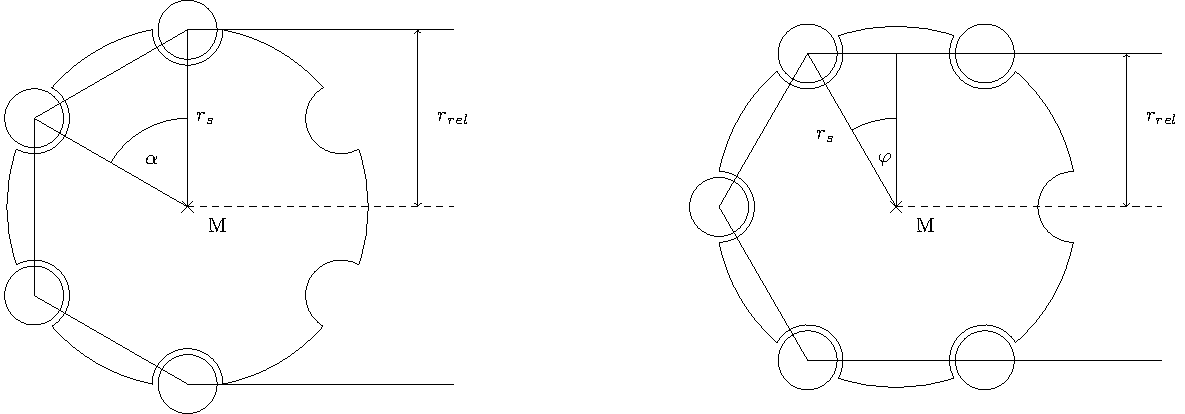
\includegraphics[width=\textwidth]{_Grafiken/Kettenrad.pdf}
    \caption{Beschreibung der Grafik}
    \label{fig:grafik}
\end{figure}
% Unterabschnitt
\section{Plots}
\begin{figure}[H]
    \centering
    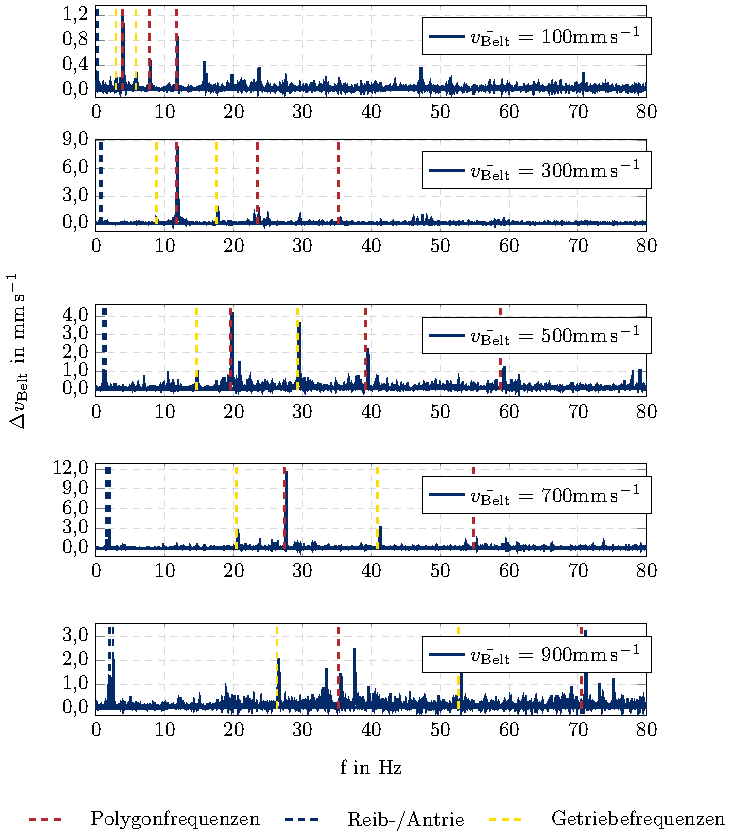
\includegraphics[width=\textwidth]{_Grafiken/FFT.pdf}
    \caption{Beschreibung der Grafik}
    \label{fig:plot1}
\end{figure}
\begin{figure}[H]
    \centering
    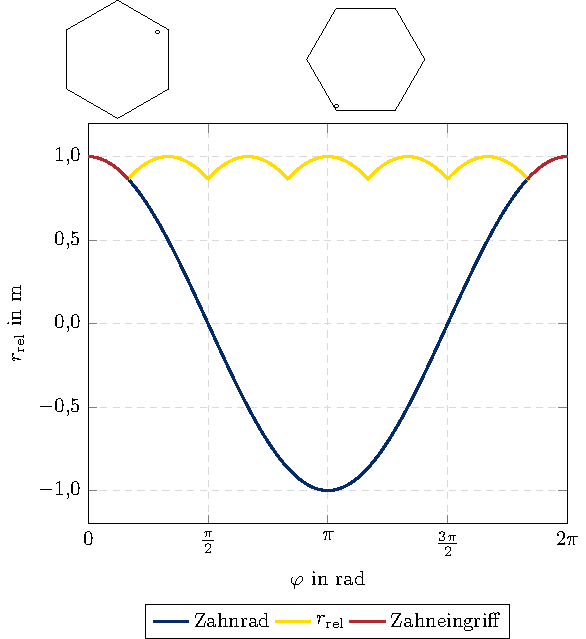
\includegraphics[width=\textwidth]{_Grafiken/Sinus.pdf}
    \caption{Beschreibung der Grafik}
    \label{fig:plot2}
\end{figure}
\subsection{Unterabschnittbschnitt}
Hier is der Unterabschnitt

\section{Noch n Abschnitt}
Noch ein Abschnitt
\chapter{Konzept}
\section{Grundlagen der Mathematik}

Die Mathematik ist eines der mächtigsten Werkzeuge in \LaTeX{}. Wir können sowohl inline-Mathematik wie $E = mc^2$ als auch Display-Mathematik verwenden.

\begin{figure}[h]
\centering
\fbox{\begin{minipage}{8cm}
Dies ist ein Platzhalter für eine Grafik.\\
Mathematische Darstellung von Konzepten
\end{minipage}}
\caption{Visualisierung mathematischer Konzepte}
\label{fig:math_visualization}
\end{figure}

\subsection{Quadratische Gleichungen}

Die allgemeine Form einer quadratischen Gleichung ist:
\[
ax^2 + bx + c = 0
\]

Die Lösungsformel lautet:
\[
x = \frac{-b \pm \sqrt{b^2 - 4ac}}{2a}
\]

\subsection{Differenzial- und Integralrechnung}

Die Ableitung einer Funktion wird definiert als:
\[
f'(x) = \lim_{h \to 0} \frac{f(x+h) - f(x)}{h}
\]

Das bestimmte Integral:
\[
\int_a^b f(x) \, dx
\]

\section{Physik}

\subsection{Klassische Mechanik}

Newtons zweites Gesetz besagt:
\[
\vec{F} = m \vec{a}
\]

Die kinetische Energie ist:
\[
E_k = \frac{1}{2}mv^2
\]

\begin{figure}[h]
\centering
\fbox{\begin{minipage}{8cm}
Grafische Darstellung von Kräften\\
und Bewegungsvektoren
\end{minipage}}
\caption{Kräfte und Beschleunigungen in der klassischen Mechanik}
\label{fig:classical_mechanics}
\end{figure}

\chapter{Beobachter}

\section{Tabellen}

\subsection{Einfache Tabelle}

\begin{center}
\begin{tabular}{|c|c|c|}
\hline
\textbf{Name} & \textbf{Fach} & \textbf{Note} \\
\hline
Alice & Mathematik & 1,0 \\
Bob & Physik & 1,5 \\
Charlie & Informatik & 1,3 \\
\hline
\end{tabular}
\end{center}

\subsection{Größere Tabelle mit Beschreibung}

\begin{center}
\begin{tabular}{|l|r|r|r|}
\hline
\textbf{Monat} & \textbf{Einnahmen} & \textbf{Ausgaben} & \textbf{Gewinn} \\
\hline
Januar & 10.000€ & 6.000€ & 4.000€ \\
Februar & 12.000€ & 7.500€ & 4.500€ \\
März & 15.000€ & 8.000€ & 7.000€ \\
April & 18.000€ & 9.500€ & 8.500€ \\
\hline
\end{tabular}
\end{center}

\section{Aufzählungen}

\subsection{Ungeordnete Liste}

\begin{itemize}
    \item Erster Punkt der Liste
    \item Zweiter Punkt mit \textbf{Formatierung}
    \begin{itemize}
        \item Verschachtelter Punkt 1
        \item Verschachtelter Punkt 2
    \end{itemize}
    \item Dritter Punkt
\end{itemize}

\subsection{Geordnete Liste}

\begin{enumerate}
    \item Erste Schritt im Prozess
    \item Zweite Schritt
    \begin{enumerate}
        \item Unterschritt A
        \item Unterschritt B
    \end{enumerate}
    \item Dritte Schritt
    \item Vierte Schritt
\end{enumerate}

\include{_Kapitel/Regler}
\include{_Kapitel/Auswertung}
\include{_Kapitel/Zusammenfassung}

% Fazit
\chapter{Fazit}
Hier kommt das Fazit hin.

\appendix

% Literaturverzeichnis ================================================================== %
\pagenumbering{Roman}
\listoffigures									% Abbildungsverzeichnis
\listoftables									% Tabellenverzeichnis
\printbibliography								% Literaturverzeichnis

% Dokumentende
\end{document}